\documentclass[10pt,color=usenames,dvipsnames]{beamer}

\usepackage{graphicx}
\usepackage{listings}

\mode<presentation> {

%\usetheme{Madrid}
\usetheme{Boadilla}

\usepackage{qrcode}
\usepackage{multirow}
\usepackage[utf8]{inputenc}

\usepackage{tikz}
\usetikzlibrary{shapes.geometric, arrows}

\usepackage[export]{adjustbox}

\definecolor{bokugreen}{rgb}{0, 0.49, 0}

%\setbeamercolor{palette primary}{fg=bokugreen}
%\setbeamercolor{palette secondary}{bg=white,fg=bokugreen}
%\setbeamercolor{palette tertiary}{bg=white,fg=bokugreen}
%\setbeamercolor{palette quaternary}{bg=white,fg=bokugreen}
\setbeamercolor{structure}{fg=bokugreen} % itemize, enumerate, etc
%\setbeamercolor{section in toc}{fg=bokugreen,bg=white} % TOC sections
\setbeamertemplate{section in toc}[sections numbered]
\setbeamertemplate{subsection in toc}[subsections numbered]


%\usebackgroundtemplate%
%{%
%	\vspace{-0.5cm}
%	\hspace{9.5cm}
%	
\includegraphics{bokulogo.png}%
%
%}

\usepackage{hyperref}
\hypersetup{%
    % warning: color makes also QR code colored, therefore commented out
	colorlinks=true,
    allcolors=bokugreen
    % Uargh! Underlining hyperrefs makes troubles with beamer's pause... :-/
    % https://tex.stackexchange.com/q/262651/8964
}

%gets rid of bottom navigation bars
\setbeamertemplate{footline}[frame number]

%gets rid of bottom navigation symbols
\setbeamertemplate{navigation symbols}{}

% Override palette coloring with secondary
%\setbeamercolor{subsection in head/foot}{bg=UBCgrey,fg=white}


%\usecolortheme{lily}
\useoutertheme{infolines}

}

\usepackage{booktabs}
\usepackage{tikz}

% Thin fonts
\usepackage{cmbright}
\usepackage[T1]{fontenc}

% add git commit hash
\usepackage{xstring}
\usepackage{catchfile}
\CatchFileDef{\HEAD}{../.git/refs/heads/master}{}
\newcommand{\gitrevision}{%
  \StrLeft{\HEAD}{7}%
}


%\definecolor{dark_grey}{gray}{0.5}
%\setbeamercolor{normal text}{fg=dark_grey,bg=white}
%\setbeamertemplate{navigation symbols}{}

%\setbeamercolor*{palette primary}{fg=gray!100,bg=gray!10}
%\setbeamercolor*{palette quaternary}{fg=gray!100,bg=gray!10}
%\setbeamercolor*{palette secondary}{fg=gray!100,bg=gray!20}
%\setbeamercolor*{palette tertiary}{fg=gray!100,bg=gray!10}
%\setbeamercolor*{navigation symbols}{fg=white,bg=white}
\usefonttheme{default}

\setbeamertemplate{blocks}[rounded][shadow=false]
%\setbeamercolor{block title}{bg=gray!10}
%\setbeamercolor{block body}{fg=gray,bg=gray!10}
%\setbeamercolor{frametitle}{fg=}

\setbeamertemplate{frametitle}[default][center]

\setbeamertemplate{itemize items}[default]
\setbeamertemplate{enumerate items}[default]

\newcommand{\F}{\mathbb{F}}

\setbeamertemplate{title page}[default][colsep=-4bp,rounded=true]
\setbeamertemplate{frametitle}[default][left]
%\addtobeamertemplate{frametitle}{}{\vspace{4em}} % increase


\title[Scientific Computing]{Scientific Computing}
\author{Peter Regner, Johannes Schmidt}
\institute{Institute for Sustainable Economic Development, BOKU, Wien}

\subtitle{Introduction}
\date{12.3.2020}
\begin{document}

% Title Page
\begin{frame}[plain]
    \maketitle
    \begin{center}
        
\includegraphics[height=1.7cm]{../common/boku-logo.pdf}\\
    \end{center}
    \vfill
    {
        \tiny
        Latest version available on
        \href{https://github.com/inwe-boku/lecture-scientific-computing/}{Github},
        this PDF is version \gitrevision.
    }
\end{frame}


\begin{frame}{Survey regarding preknowledge}
    \begin{center}
        \textcolor{black}{
            \qrcode[height=4.5cm]{https://www.menti.com/}
        }\\
        \vspace{0.5cm}
        \huge{
            menti.com
        }
    \end{center}
\end{frame}

\begin{frame}

	\tableofcontents

\end{frame}

\section{Who we are}

\begin{frame}{Who we are}
    Johannes Schmidt <johannes.schmidt@boku.ac.at>\\
    \begin{itemize}
        \item Associate Prof. in Energy \& Resource Economics at the Institute for Sustainable Economic Development
        \item Works on modeling of renewable energy systems in R, GAMS (and Python)
        \item Studied Computer Science at TU Wien
    \end{itemize}

    \pause
    \bigskip

    Peter Regner <peter.regner@boku.ac.at>
    \begin{itemize}
        \item PhD student at the Institute for Sustainable Economic Development
        \item Worked almost 7 years as Python developer in semiconductor industry
        \item Studied mathematics at TU Wien
    \end{itemize}
\end{frame}

\section{What this course is about}

\begin{frame}{Aim of course}

	Learn to use programming as a tool in research

	\begin{itemize}
		\item Version control your code with Git and collaborate on Git(hub)
		\item Install Python, Python packages, and Jupyter notebook servers in Conda environments
		\item Start programming in python and understand flow features (loops and conditions) and functions
		\item Get an overview of the Python scientific ecosystem
		\item Use Python scientific stack packages (numpy, xarray)
		\item Use open (climate) data in your research projects
		\item Generate plots using matplotlib
	\end{itemize}

\end{frame}

\begin{frame}{Example use cases}

	Possible homework/application of presented know-how:\\

    Mean wind speed and wind turbine locations in the US

    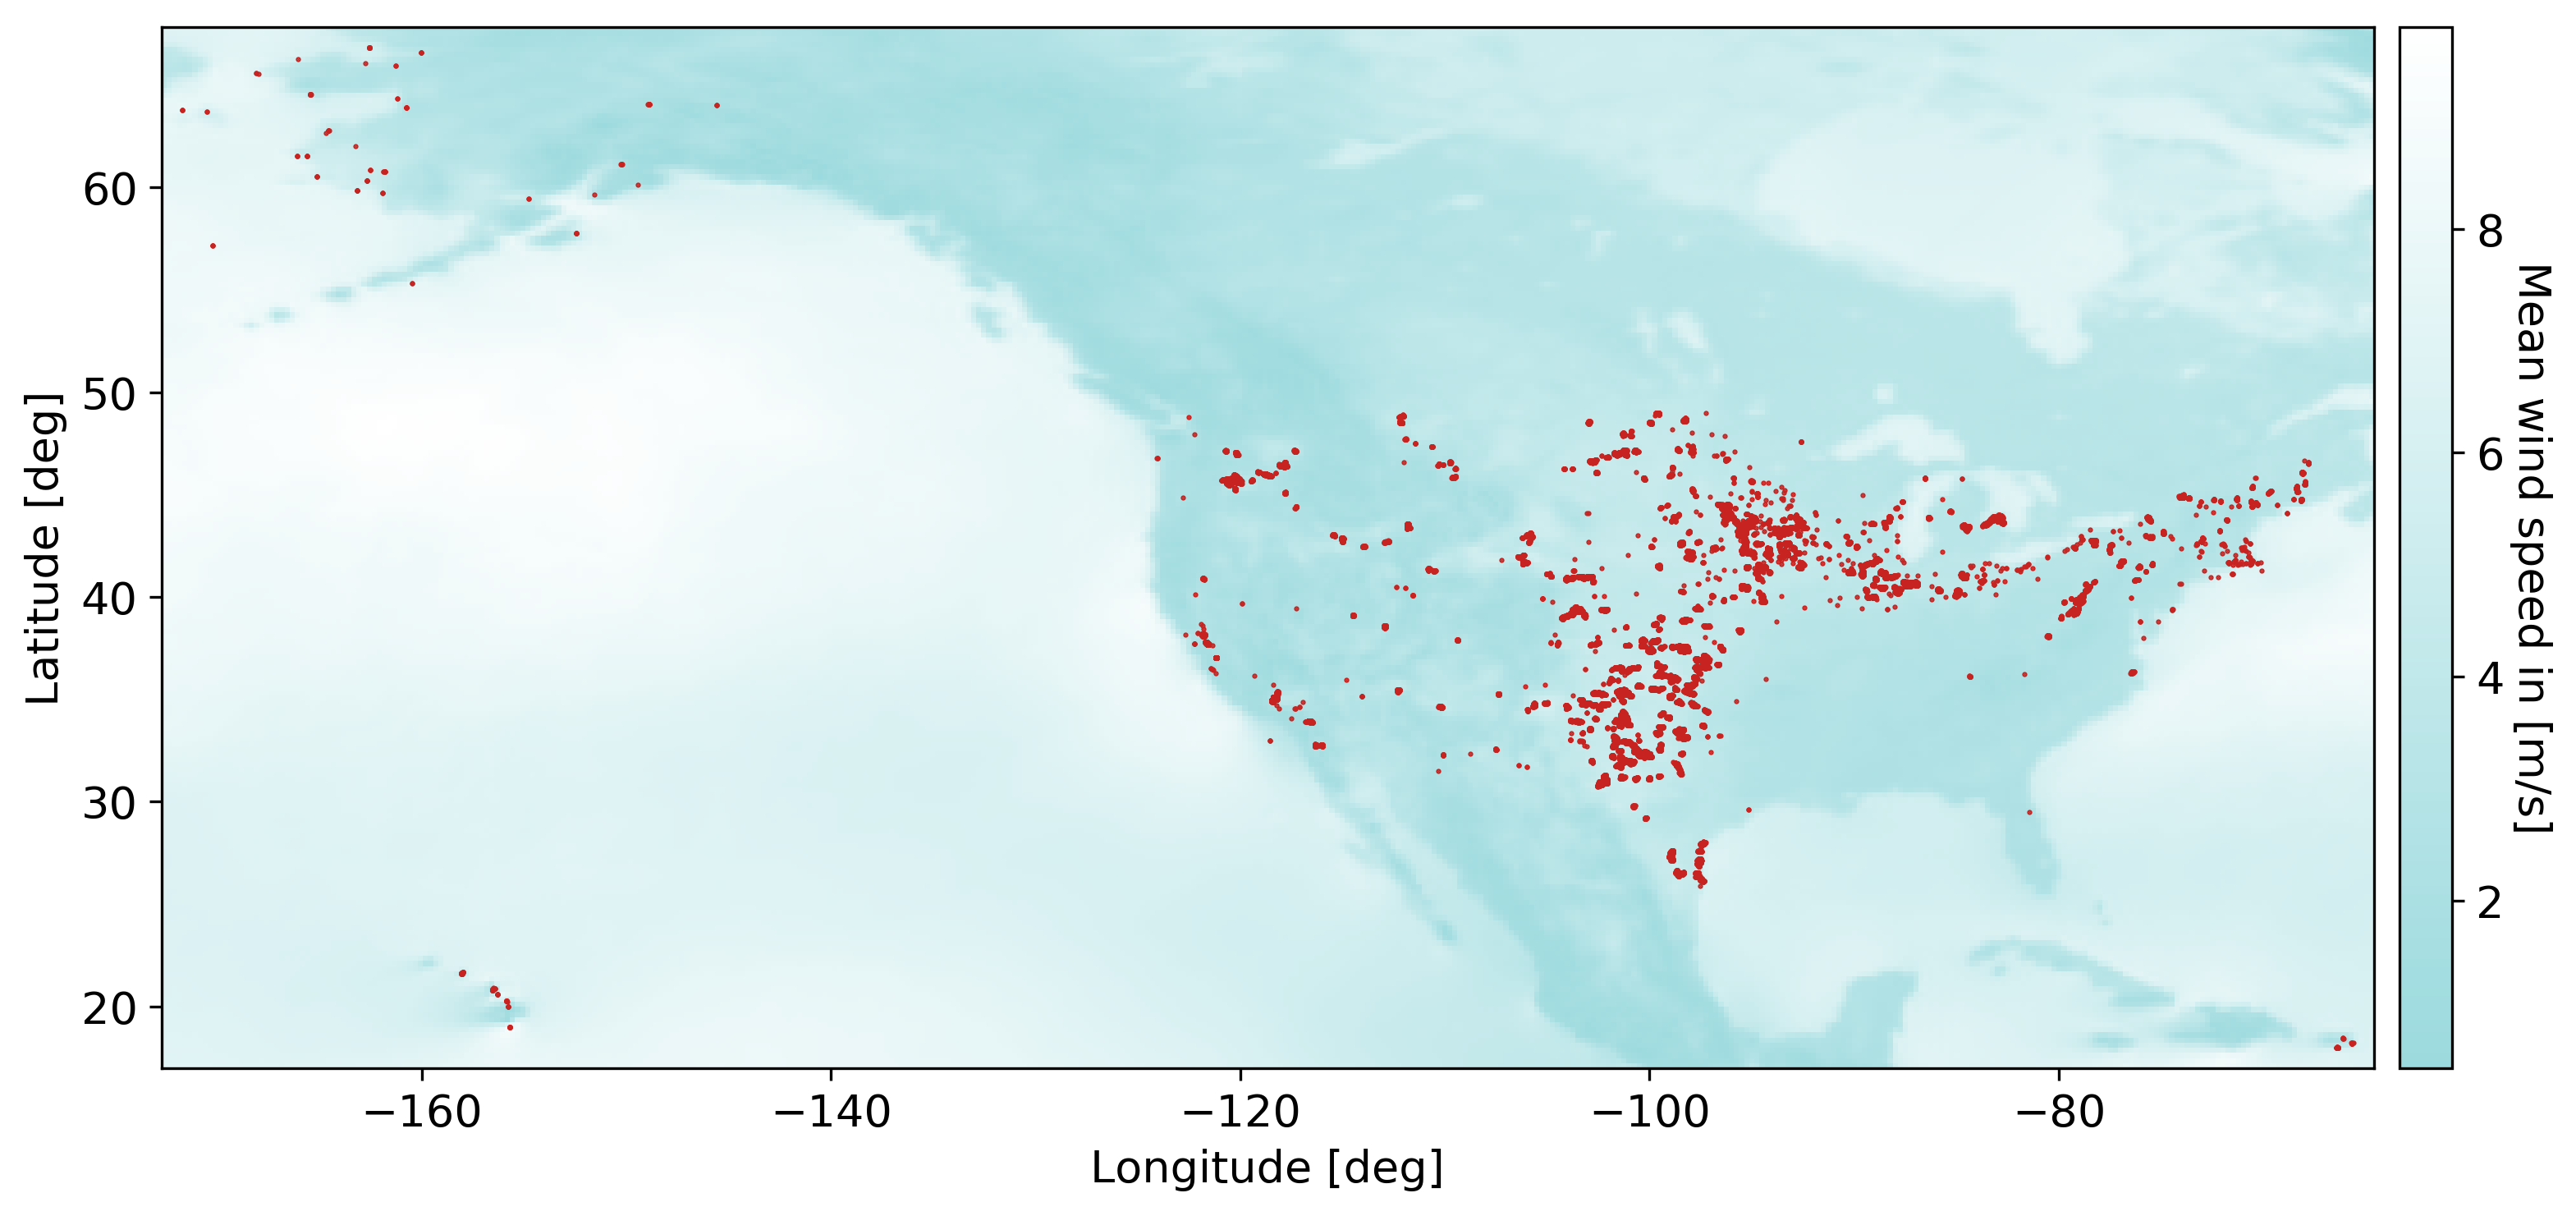
\includegraphics[width=\textwidth]{mean_wind_speed_and_turbines.png}\\

\end{frame}

\section{How the class works}

\begin{frame}{How the class works}
	\begin{itemize}
		\item 1.5 hours of lecture
		\item 1.5 hours of practical exercises
		\item Homework in groups
	\end{itemize}
\end{frame}

\begin{frame}{Dates}

	\begin{table}

	\begin{tabular}{|c|c|}
		\hline
		Date&Content\\
		\hline
		12.03.2020	13:00-16:15	& Introduction \\

		19.03.2020	13:00-16:15&Introduction to Git\\

		26.03.2020	13:00-16:15&Installation of Python in Conda\\

		02.04.2020	13:00-16:15&Start programming in Python\\

		30.04.2020	13:00-16:15&Python scientific ecosystem\\

		07.05.2020	13:00-16:15&Numpy and xarray, \textbf{Maybe skipped}\\

		14.05.2020	13:00-16:15& Use open (climate) data\\

		28.05.2020	13:00-16:15&Generate plots using matplotlib\\

		04.06.2020  13:00-16:15&\textbf{Replacement date for 7th of May}\\
		\hline
	\end{tabular}
\end{table}

\end{frame}


\section{Prerequisites}

\begin{frame}{Prerequisites}
	\begin{itemize}
        \item You should feel very comfortable with your respective operating system (Windows, Linux, Mac OS)
		\item Ideally, you have some experience with using a command line / terminal
		\item In a perfect world, you have programmed before
	\end{itemize}
\end{frame}


\section{How we grade}

\begin{frame}{Grading scheme}

	\begin{itemize}
		\item Organize in groups of 4 students
		\item Do homework together
		\item Be prepared to present homework individually ("Kreuzerlübung")
	\end{itemize}

\end{frame}

\section{Resources}

\begin{frame}[fragile]{Resources}
    Slides, links and other material in this Github repository:
    \href{https://github.com/inwe-boku/lecture-scientific-computing}{https://github.com/inwe-boku/lecture-scientific-computing}\\
    \bigskip
    \pause
    Where/whom to ask questions?
	\begin{itemize}
        \item In a new Github issue, do not write emails to us:
            \href{https://github.com/inwe-boku/lecture-scientific-computing/issues}{https://github.com/inwe-boku/lecture-scientific-computing/issues}
		\item Your fellow peers in your group
		\item Ask us during class
	\end{itemize}
\end{frame}

\section{First assignment}

\begin{frame}{First assignment (I)}

Homework (due on 19th of March):

\begin{itemize}
	\item register at github.com or any alternative GIT hoster (e.g. gitlab.com)
	\item install a GIT and gitk (see instructions (1) on next slide)
	\item click/browse quickly through links \& tutorials (see on next slide)
	\item clone a repository, change a file and commit (see instructions (2) next slide)
	\item prepare one question about GIT and add it to the list: \href{https://yourpart.eu/p/lecture-scientific-computing}{https://yourpart.eu/p/lecture-scientific-computing}

\end{itemize}


\end{frame}

\begin{frame}[fragile]{First assignment (II)}
	(1) Install GIT \& gitk

    {\bf Installation on Linux:}\\
    on Debian based systems run the command:

	\begin{verbatim}
	    sudo apt install git gitk
	\end{verbatim}

    {\bf Installation on Windows:}
    \begin{enumerate}
        \item install notepad++ (\href{https://notepad-plus-plus.org/downloads/}{https://notepad-plus-plus.org/downloads/})
        \item install git for windows
            (\href{https://gitforwindows.org/}{https://gitforwindows.org/}). During the
            installation procedure, choose notepad++ as your preferred editor.
    \end{enumerate}

    {\bf Configure name and mail address:}\\
    Run a terminal (windows: GIT bash) and run the command\footnote{
        See also
            \href{https://git-scm.com/book/en/v2/Getting-Started-First-Time-Git-Setup}
            {https://git-scm.com/book/en/v2/Getting-Started-First-Time-Git-Setup}
    }:
    {\small
        \begin{verbatim}
    git config --global user.name "My Name or Pseudonym"
    git config --global user.email my-public-mailadress@example.com
        \end{verbatim}
    }

\end{frame}

\begin{frame}[fragile]{First assignment (III)}
	(2) Clone the lecture repository and add a commit

	Run a terminal (windows: GIT bash) and run the command:

    {\small
        \begin{verbatim}
    git clone https://github.com/inwe-boku/lecture-scientific-computing
        \end{verbatim}
    }

	Then edit any arbitrary file, e.g. add "I was here" to REDAME.md and run:

	\begin{verbatim}
    cd lecture-scientific-computing
	    git add path/to/file-you-changed
	    git commit -m 'I changed a file'
	\end{verbatim}

	Explain your change in the commit message and close the editor.

	Run gitk to check your commit.

\end{frame}

\begin{frame}[fragile]{First assignment (IV)}
	See also:\\
	\href{https://guides.github.com/introduction/git-handbook/}{https://guides.github.com/introduction/git-handbook/}\\
	(especially the section "Example: Contribute to an existing repository")
    \bigskip

	More helpful resources about GIT can be found here:\\
	\href{https://github.com/inwe-boku/lecture-scientific-computing/blob/master/lecture01-git-version-control/links.rst}
	{https://github.com/inwe-boku/lecture-scientific-computing/blob/master/lecture01-git-version-control/links.rst}
\end{frame}

\begin{frame}{First assignment (V)}
    Warning: you will need to push your homework to a public Github repository. Your Github account
    is your business card for programmers -- your homework will be part of it. You can create a
    separate Github account only for this course to be anonymous or your group deletes the
    repository after the semester, if you don't want your homework to remain public. Note: the name
    and mail address chosen during the GIT installation will be public too.
\end{frame}

\end{document}

